\documentclass[tikz,border=2pt]{standalone}
\usepackage[T1]{fontenc}
\usepackage{libertine}
\usepackage{xcolor}
\usetikzlibrary{arrows.meta,shapes.geometric}

\begin{document}
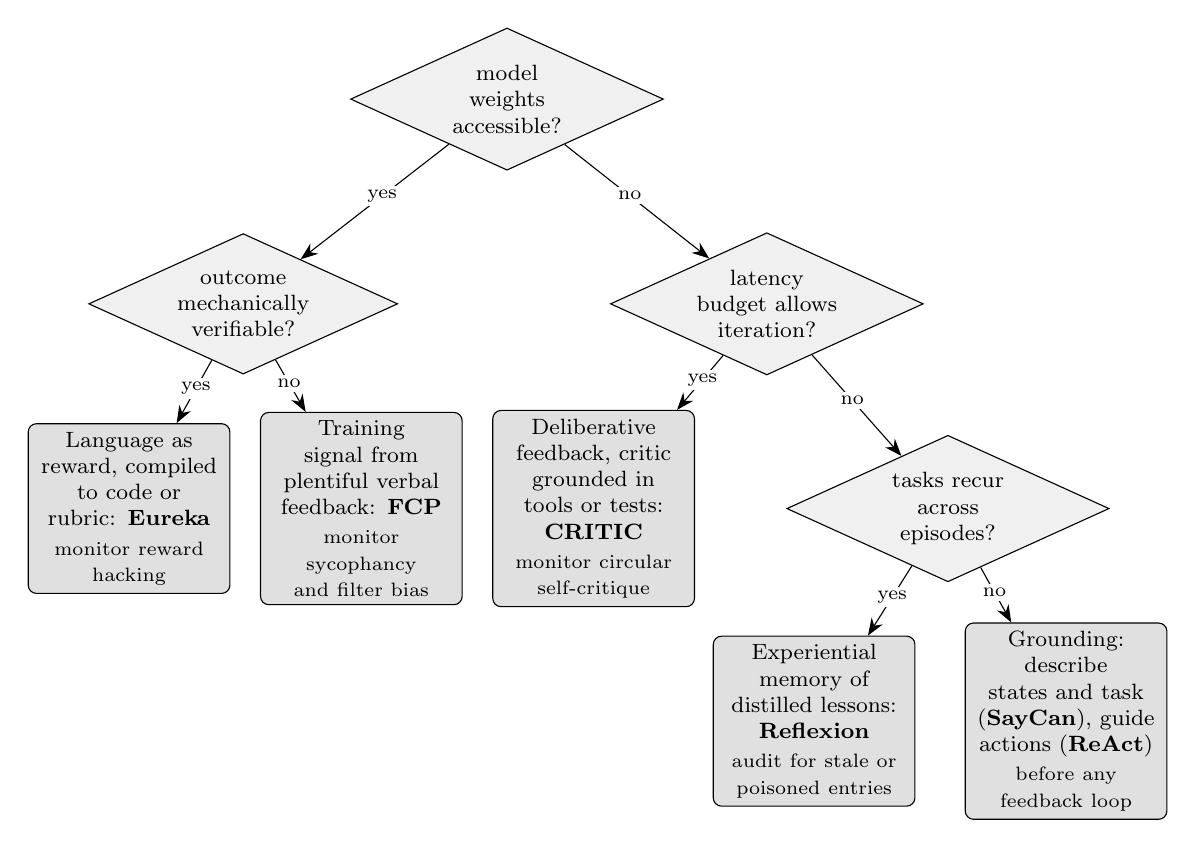
\begin{tikzpicture}[
    font=\footnotesize,
    >={Stealth[length=2.2mm]},
    every node/.append style={execute at begin node={\hyphenpenalty=10000\exhyphenpenalty=10000\relax}},
    decision/.style={diamond, aspect=2.2, draw, align=center,
        inner sep=1pt, text width=1.85cm, fill=black!6},
    leaf/.style={rectangle, rounded corners=3pt, draw, align=center,
        inner sep=3pt, text width=2.35cm, fill=black!12},
    ans/.style={font=\scriptsize, fill=white, inner sep=1.5pt}
]
    \node[decision] (d1) at (6.2,0)      {model weights accessible?};
    \node[decision] (d2) at (2.85,-2.6)  {outcome mechanically verifiable?};
    \node[decision] (d3) at (9.5,-2.6)   {latency budget allows iteration?};
    \node[decision] (d4) at (11.8,-5.2)  {tasks recur across episodes?};

    \node[leaf] (l1) at (1.4,-5.2)  {Language as reward, compiled to code or rubric: \textbf{Eureka}\\[1pt]{\scriptsize monitor reward hacking}};
    \node[leaf] (l2) at (4.35,-5.2) {Training signal from plentiful verbal feedback: \textbf{FCP}\\[1pt]{\scriptsize monitor sycophancy and filter bias}};
    \node[leaf] (l3) at (7.3,-5.2)  {Deliberative feedback, critic grounded in tools or tests: \textbf{CRITIC}\\[1pt]{\scriptsize monitor circular self-critique}};
    \node[leaf] (l4) at (10.1,-7.9) {Experiential memory of distilled lessons: \textbf{Reflexion}\\[1pt]{\scriptsize audit for stale or poisoned entries}};
    \node[leaf] (l5) at (13.3,-7.9) {Grounding: describe states and task (\textbf{SayCan}), guide actions (\textbf{ReAct})\\[1pt]{\scriptsize before any feedback loop}};

    \draw[->] (d1) -- node[ans, pos=0.45] {yes} (d2);
    \draw[->] (d1) -- node[ans, pos=0.45] {no}  (d3);
    \draw[->] (d2) -- node[ans, pos=0.45] {yes} (l1);
    \draw[->] (d2) -- node[ans, pos=0.45] {no}  (l2);
    \draw[->] (d3) -- node[ans, pos=0.45] {yes} (l3);
    \draw[->] (d3) -- node[ans, pos=0.45] {no}  (d4);
    \draw[->] (d4) -- node[ans, pos=0.45] {yes} (l4);
    \draw[->] (d4) -- node[ans, pos=0.45] {no}  (l5);
\end{tikzpicture}
\end{document}
